\documentclass[14pt]{article}
\usepackage[margin=1in]{geometry}
\usepackage{amsmath}
\usepackage{amssymb}
\usepackage{fancyhdr}
\usepackage{graphicx}
\usepackage{xcolor}
\usepackage{hyperref}
\renewcommand{\familydefault}{\sfdefault}
\parindent 0ex
\everymath{\displaystyle{}}
\author{Andy Smit}
\title{ENGG 225\\Fundamentals of Electrical Circuits and Machines}
\date{Winter 2019}


\begin{document}
    \maketitle
    \section{Introduction}
    \subsection{Electric Circuits:}
    The interconnection of circuit elements in a closed path by
    conductors. The concept of electrical charge is the basics for
    describing all electrical phenomena. Charge exists in discrete
    quantities of integer multiples of $1.60\times 10^{-19}C$. In
    circuit analysis there are two fundamental electrical quantities
    voltage and current. 
    \subsection{Electical Current:}
    Electrical current is defined as the rate of flow of electrical
    charges.
    $$i(t)=\frac{d q(t)}{dt}$$ It is assumed that $i$ is a measure of
    the equivalent flow of positive charge flow. Given $i(t)$, we can
    also find $q(t)$
    $$q(t)=\int\limits_{t_0}^t i(t)\, dt+q(t_0)$$ Normally there is an
    assigned reference direction for current. Often the direction is
    unknown and is assumed. The actual direction is determined by the
    sign of $i$
    \subsubsection{Direct and Alternating Current:}
    \begin{figure}[h]
        
\includegraphics[width=0.45\textwidth]{DirCur.eps}
        \hspace{0.09\textwidth}
        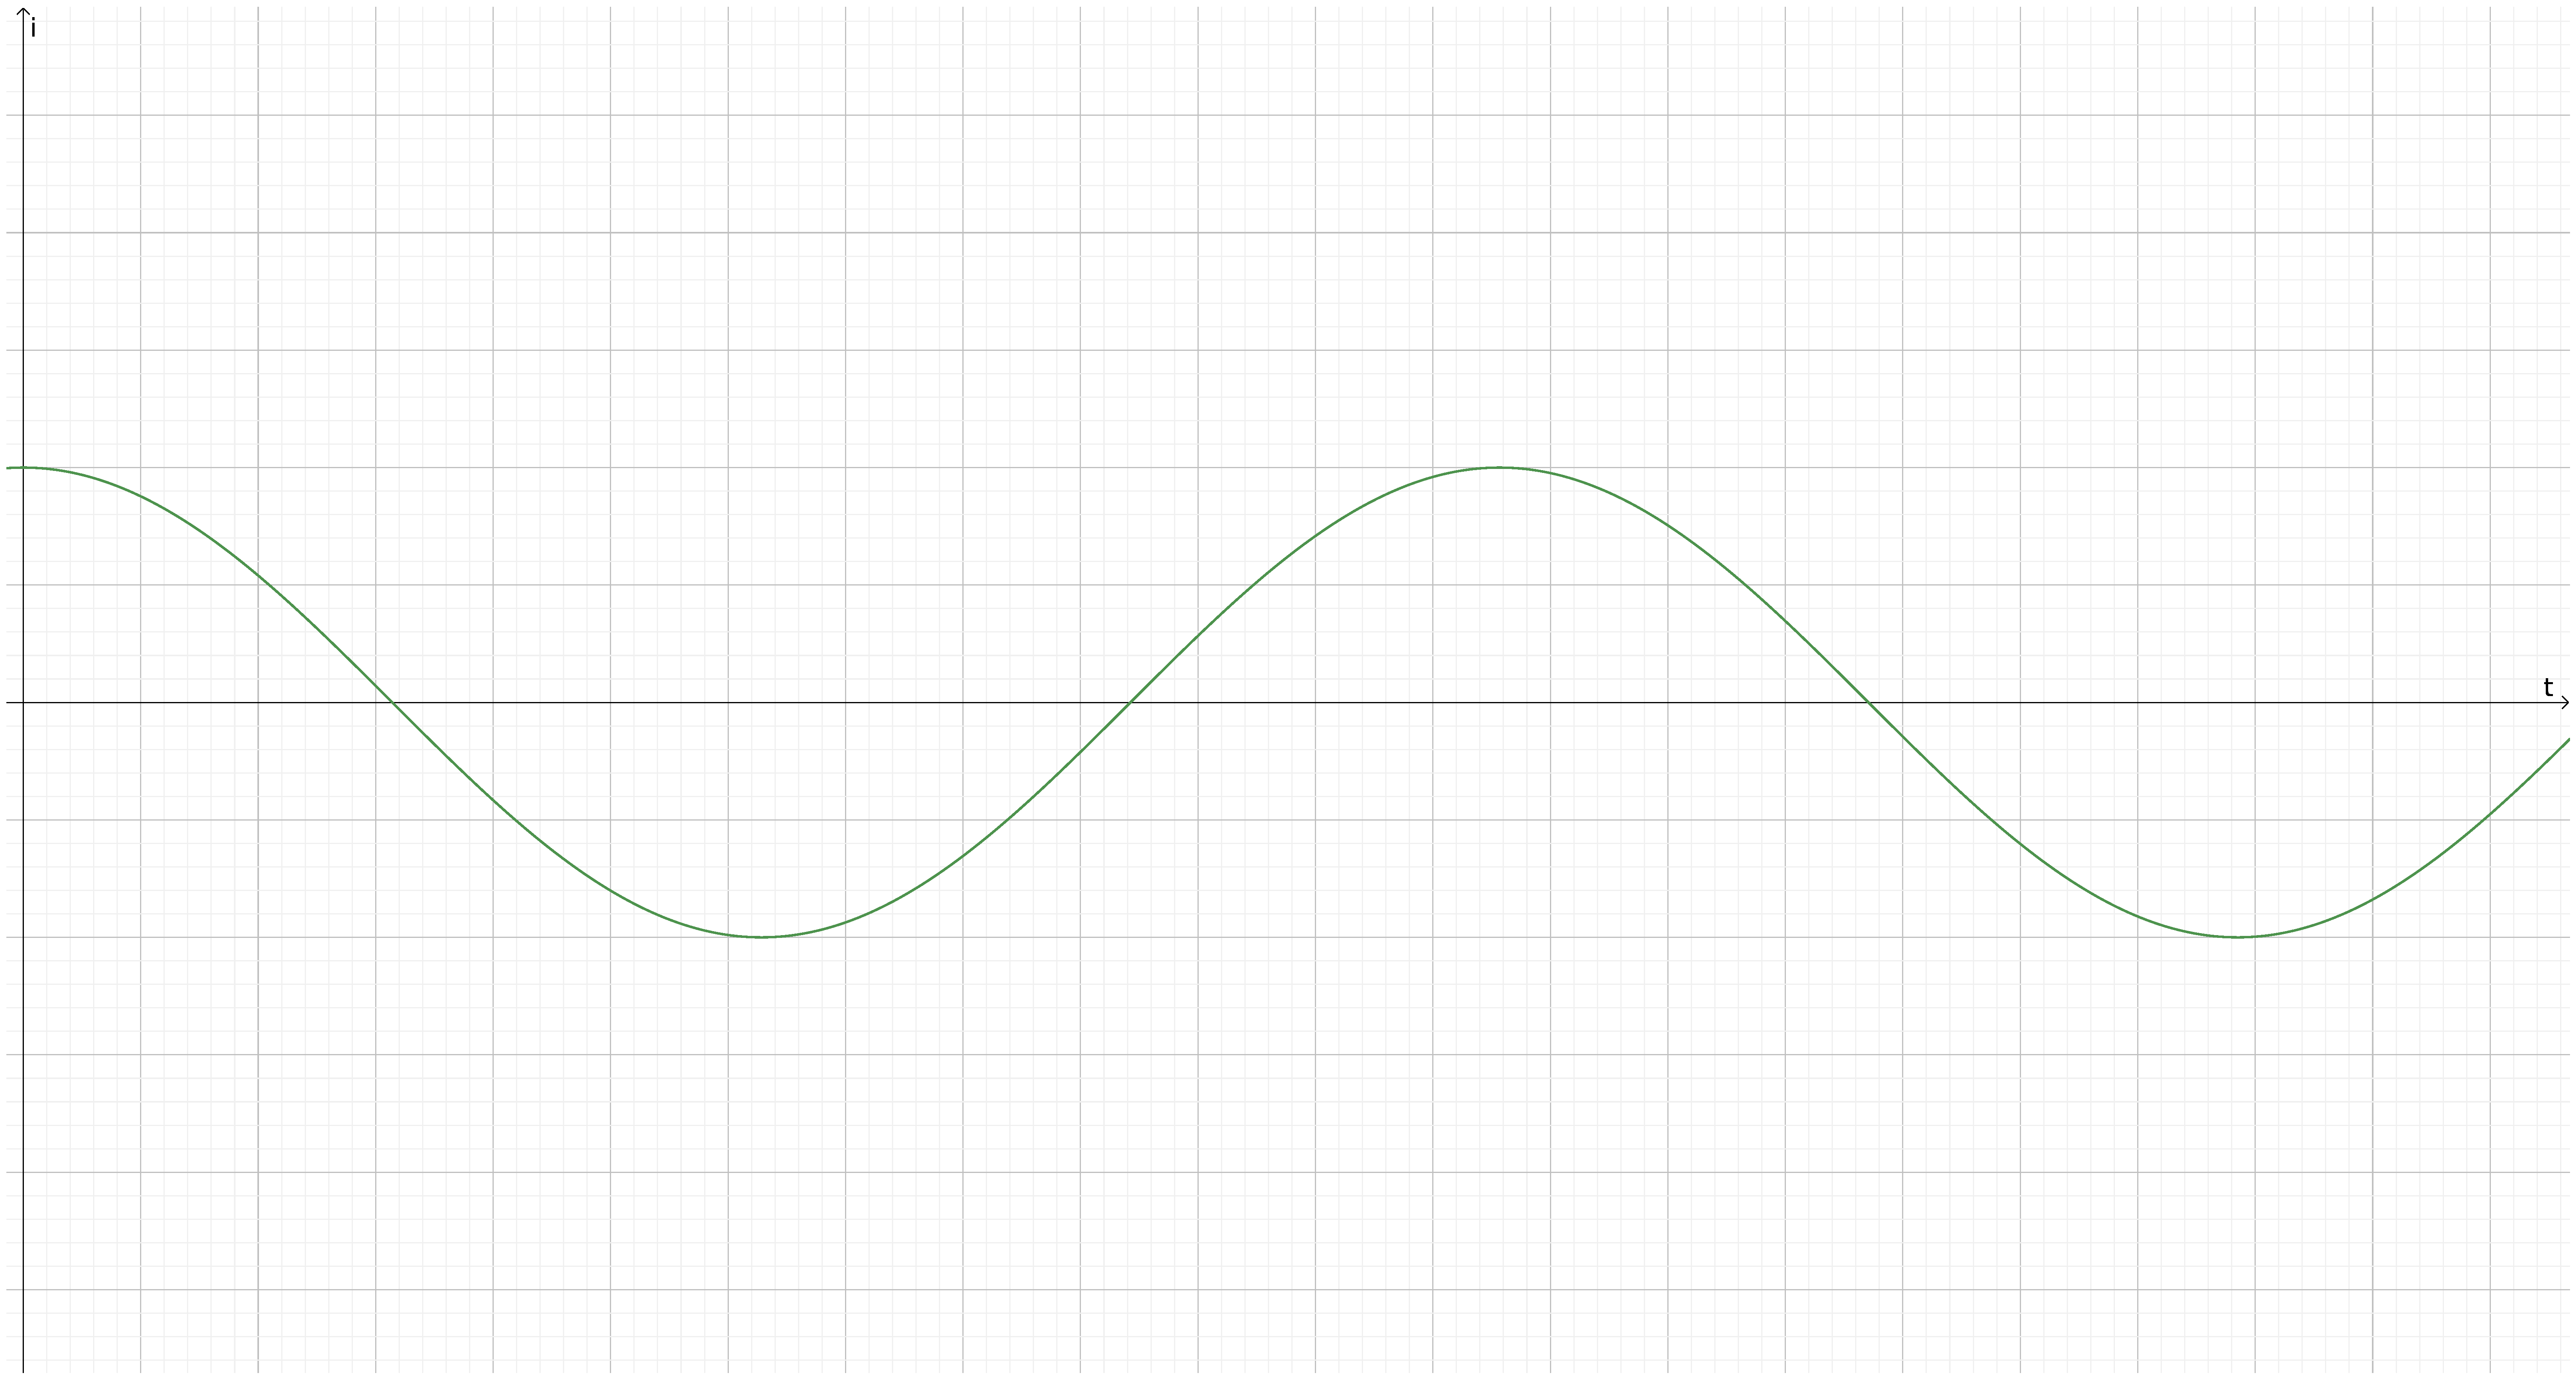
\includegraphics[width=0.45\textwidth]{AltCur.eps}
        \caption{Direct and Alternating Current}
    \end{figure}
    \subsubsection{Notation for Current}
    \subsection{Voltage}
    Voltage is the energy transferred to or from a circuit element per
    unit of charge that flows through it. 
    $$V(t)=\frac{dw(t)}{dq(t)}$$ Voltage is often thought of as the
    potential difference across a circuit element. The polarity of the
    voltage is used to determine which node of a circuit element is at a
    higher potential then the other. If a circuit element has two nodes
    $a$ and $b$ with a voltage $V$ across it such that $a$ is the
    negative terminal and $b$ is the positive terminal then it can be
    said that $b$ is $V$ volts higher in potential then $a$. For
    analysis purposes, reference polarities can be assigned if they are
    not given. The reference polarities can be chosen arbitrarily and if
    the actual polarity is the opposite the value of $V$ is negative. 
    \subsection{Ideal Circuit Elements:}
    All circuit elements are characterized by the voltage current
    relationship they hold.
    \subsubsection{Ideal Conductor:}
    An ideal conductor is a conductor with $0$ resistance; this implies
    that the current through the conductor stays constant, and there is
    $0$ voltage drop across the conductor, or $R=0\Omega$, $\Delta
    i=0A$, and $V=0V$. The components on either side of the conductor
    are treated as if they are shorted (connected) together. The absence
    of a conductor is an open circuit. Since all conductors are ideal,
    they can be as arbitrarily long or short as necessary as long as the
    connection remains the same. 
    \subsubsection{Sources:}
    \begin{enumerate}
        \item Independent Voltage Sources:\\
        Tells which terminal is at a higher potential voltage and by
        what amount. The current is unknown and is dependent on the
        circuit the voltage source is connected to. A voltage source can
        be either AC or DC
        \item Dependent Voltage Source:\\
        The voltage provided by a dependent voltage source is based on
        some other value in the circuit. The voltage current
        characteristics are the same as a independent voltage source,
        except the value of the voltage provided depends on a voltage or
        current elsewhere in the circuit. 
        \item Independent Current Source:\\
        Tells the exact value of the current flowing through it. The
        current provided is unaffected by other elements in the circuit,
        but the voltage is dependent on the circuit connected to the
        source.
        \item Dependent Current Source:\\
        A dependent current source has the same properties as an
        independent current source except the current is dependent on
        the current or voltage in another element of the circuit.
    \end{enumerate} 
    \subsubsection{Resistors}
    Resistors resist the flow of current by causing a drop in voltage.
    The relationship between the voltage across a resister and the
    current through the resistor is given by Ohm's Law. Ohm's Law states
    that if the current through a resistor is shown in the direction of
    the voltage drop then the voltage is given by $$V=i\,R$$ where $V$
    is the voltage measured in volts $V$, $i$ is the current measured in
    amperes (amps) $A$ and $R$ is the resistance of the resistor
    measured in ohms $\Omega$. If the current through a resistor is
    shown in the direction of the voltage rise then ohms law states
    $$V=-i\,R$$ Likewise Ohms Law states that the current through a
    resistive element is 
    $$i=\frac{1}{R}V$$ The quantity $G=\frac{1}{R}$ is referred to as
    the conductance of a circuit element. Conductance is measured in
    units of Siemens $\Omega^{-1}$
    \subsection{Power and Energy}
    Power is given as the change in energy $W$ over a change in time $t$
    $$P=\frac{dW}{dt}$$ In electric circuits, power can be given as the
    product of voltage and current
    $$P=V\, i$$ Power is measured in watts where $1W=1J/s$. If current
    is labelled in the direction of a voltage drop over an element
    (passive reference direction) which implies the element is absorbing
    power then use
    $$P=V\, i$$ If the current is labelled in the direction of a voltage
    increase then use 
    $$P=-V\,i$$ In both cases, if $P>0$ then the element is absorbing
    power, and conversely if $P<0$ the element is supplying power.
    \subsubsection{Power in Resistors}
    As stated above power in a circuit element is given by 
    $$P=V\, i$$ if it is absorbing power. However voltage and current
    are related by Ohms Law for a resistive circuit element. From Ohms
    law the following is obtained,
    $$V=i\, R$$
    \begin{align*}
        \therefore && P=i^2R && P=\frac{V^2}{R}
    \end{align*}
    As $i^2\geq0$, $V^2\geq0$ and $R>0$ for any resistor necessarily
    $P\geq0$ for any resistor.
    \subsubsection{Energy}
    As stated above
    \begin{align*}
        P&=\frac{dW}{dt}\\
        \therefore W=\int\limits_{t_1}^{t_2}P(t)dt
    \end{align*}
    \subsection{Kirchoff's Laws}
    \subsubsection{Kirchoff's Current Law (KCL)}
    Consider a node in a circuit. The total current flowing into the
    node is equal to the current out, or the algebraic sum of all
    currents at a node must be 0.
    $$\sum i_n=0$$ The convention used will be add all currents entering
    the node and subtract currents leaving the node. In the node voltage
    method the opposite convention is used.
    \subsubsection{Kirchoff's Voltage Law (KVL)}
    Kirchoff's voltage law states the algebraic sum of the voltages
    equals 0 for any closed path in an electric circuit.
    $$\sum V_n=0$$ When summing voltages around a loop the direction of
    the loop is arbitrary. If the loop crosses the positive terminal of
    an element add $V$. Conversely if the loop crosses the negative
    terminal of an element subtract $V$.
    \subsection{Series and Parallel Circuits}
    \subsubsection{Series Circuits}
    Two elements are in series if they are connected at one node only
    and there is no other element connected to that node. Elements in
    series have the same current and direction of current.
    \subsection{Parallel Circuits}
    Two elements are in parallel if their terminals are directly
    connected to each other. In other words they are connected to the
    same two nodes. Elements in parallel must have the same actual
    voltage.
    \section{Resistive Circuits}
    \subsection{Series and Parallel Resistance}
    \subsubsection{Series Resistance}
    A series combination of resistors has an equivalent resistance equal
    to the sum of the original resistances. For $n$ resistors of
    resistance $R_k$, the equivalent resistance $R_{eq}$ is given by,
    $$\sum\limits_{k=1}^nR_k=R_{eq}$$
    \subsubsection{Parallel Resistance}
    A parallel combination of resistors has an equivalent resistance
    equal to the reciprocal of the sum of the reciprocal of the original
    resistances. For 2 resistors of resistance $R_1$ and $R_2$ in
    parallel the equivalent resistance $R_{eq}$ is given by
    $$R_{eq}=\frac{R_1R_2}{R_1+R_2}$$ From the above result it is show
    able that for two resistors of resistance $R$ in parallel have an
    equivalent resistance 
    $$R_{eq}=\frac{1}{2}R$$ More generally for $n$ resistors of
    resistance $R_k$, the equivalent resistance $R_{eq}$ is given by
    $$\frac{1}{R_{eq}}=\sum\limits_{k=1}^n\frac{1}{R_k}$$ or
    $$R_{eq}=\frac{1}{\sum\limits_{k=1}^n\frac{1}{R_k}}$$
    \subsection{Voltage and Current Division}
    \subsubsection{Voltage Division}
    In a series connection of resistors, the total voltage across the
    series branch of resistors divides among the resistors proportional
    to their size. For $n$ resistors of resistance $R_m$ with a total
    voltage across them of $V$ the voltage in the $k^{th}$ resistor
    $V_k$ is given by
    $$V_k=\frac{R_k}{\sum\limits^nR_m}V$$
    \subsection{Current Division}
    In a parallel connection of resistors, the total current available
    to the parallel resistor divides among them inversely proportionally
    to their size. For 2 resistors of resistance $R_1$ amd $R_2$ and a
    total current of $i$ then the current $i_1$ through $R_1$ is
    $$i_1=\frac{R_2}{R_1+R_2}$$
    \subsection{Node Voltage Analysis}
    The node voltage method allows analysis of any circuit where other
    methods may fail. The node voltage method follows the following
    steps
    \begin{enumerate}
        \item Identify nodes and known node voltages
        \item Apply KCL at nodes; Develop a system of equations where
        the unknowns are the node voltages
        \item Solve system of equations to determine node voltages.
    \end{enumerate}
    A node voltage is the potential difference between a node and the
    reference node. If a voltage source exists the negative terminal of
    the node should be chosen as the reference (ground) node. 
    \section{Operational Amplifiers}
    \section{Capacitors and Inductors}
    \section{Sinusoidal Currents and Voltages}
    \section{DC Machines}  
\end{document}